\documentclass[10pt, handout, xcolor=table]{beamer}

\usepackage[utf8]{inputenc}
\usepackage{amsmath}
\usepackage{amsfonts}
\usepackage{amssymb}
\usepackage{mathtools}
\newcommand*\themecol{\usebeamercolor[fg]{structure}}

\setbeamertemplate{navigation symbols}{}
 \setbeamertemplate{footline}[frame number]

\newcommand{\overbar}[1]{\mkern 1.5mu\overline{\mkern-1.5mu#1\mkern-1.5mu}\mkern 1.5mu}

\usepackage{tikz}
\usetikzlibrary{shapes.geometric, arrows}
\tikzstyle{prob} = [rectangle, minimum width=3cm, text width = 4.5cm, minimum height=1cm, text centered, draw=black, fill= blue!20]
\tikzstyle{stat} = [rectangle, minimum width=3cm,  text width = 4.5cm, minimum height=1cm, text centered, draw=black, fill= red!20]
\tikzstyle{arrow} = [thick,->,>=stealth]

\DeclarePairedDelimiter\abs{\lvert}{\rvert}%
\DeclarePairedDelimiter\norm{\lVert}{\rVert}
\DeclarePairedDelimiter\ceil{\lceil}{\rceil}
\DeclarePairedDelimiter\floor{\lfloor}{\rfloor}



\setlength{\parindent}{0pt}
\setlength{\parskip}{6pt}


\title{STAT 111\\
{\small Recitation 9}}

\author{Mo Huang}
\institute{Email: mohuang@wharton.upenn.edu \\
\vspace{0.25cm}
Office Hours: Wednesdays 3:00 - 4:00 pm, JMHH F96\\
\vspace{0.25cm}
Slides (adapted from Gemma Moran): \url{github.com/mohuangx/STAT111-Fall2018} }


\date{November 9, 2018}


\begin{document}

\begin{frame}
\titlepage
\end{frame}

\begin{frame}{Hypothesis Tests for the Mean}
\begin{itemize}
\setlength{\itemsep}{8pt}
\item Same process as before but we need to be careful about our test-statistic.
\item Let $X_1, \dots, X_n$ be i.i.d random variables with (unknown) mean $\mu$ and (unknown) variance $\sigma^2$.
\item Set $H_0: \mu = \mu_0$ and $H_1$ for some number $\mu_0$ and choose $\alpha$.
\item Determine test-statistic... \\[5pt]
\begin{itemize}
\setlength{\itemsep}{8pt}
\item We know under the null,  $\overline{X} \sim N(\mu_0, \frac{\sigma^2}{n})$ for large $n$.
\item But we don't know $\sigma^2$! Calculate $s^2$ (the sample variance).
\item Standardize:
$$T = \frac{\overline{X} -\mu_0}{s/\sqrt{n}}$$
\item It turns out $T$ is not normally distributed so can not use $z$-chart! It is $t$-distributed with $n-1$ ``degrees of freedom''.
\end{itemize}
\end{itemize}
\end{frame}

\begin{frame}{The $t$-distribution}
\begin{itemize}
\setlength{\itemsep}{7pt}
\item Similar to the normal distribution, but with heavier tails.
\item This is to account for the uncertainty in not knowing $\sigma^2$.
\item As $n$ gets bigger, the estimate $s^2$ is better and the $t$-distribution gets closer to the normal distribution. When $n = \infty$, the $t$-distribution becomes the normal distribution.
\item This is why we need the ``degrees of freedom''.
\end{itemize}
\begin{figure}
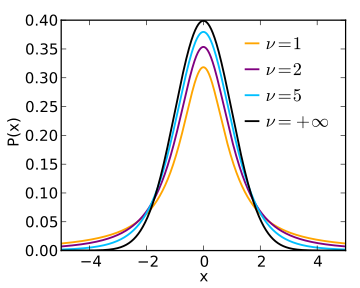
\includegraphics[width = 0.4\textwidth]{images/rec11_1}
\caption{Credit: Wikipedia. $\nu$ is degrees of freedom.}
\end{figure}
\end{frame}

\begin{frame}{Example}
\begin{itemize}
\setlength{\itemsep}{8pt}
\item A chocolate block is advertised as being 8 oz. Suppose we are concerned that the chocolate manufacturers are giving us less than 8 oz of chocolate in a block.  We collect 15 blocks of chocolate and calculate:
$$\bar{x} = 7.88, \quad s^2 = 0.06.$$
\item<1->[Step 1] $H_0: \mu = 8$ vs. $H_1: \mu < 8$.   
\item<2->[Step 2] Choose $\alpha = 0.05$. 
\item<3->[Step 3] Test-statistic is 
$$t = \frac{\bar{x} - \mu_0}{s/\sqrt{n}} = \frac{7.88 - 8}{\sqrt{0.06/15}} = -1.90$$
\item<4->[Step 4]  Find the critical region.
%\item<5->[Step 5] Reject $H_0$ as $p$-value is less than 0.05.
\end{itemize}
\end{frame}

\begin{frame}{Example}
\begin{figure}
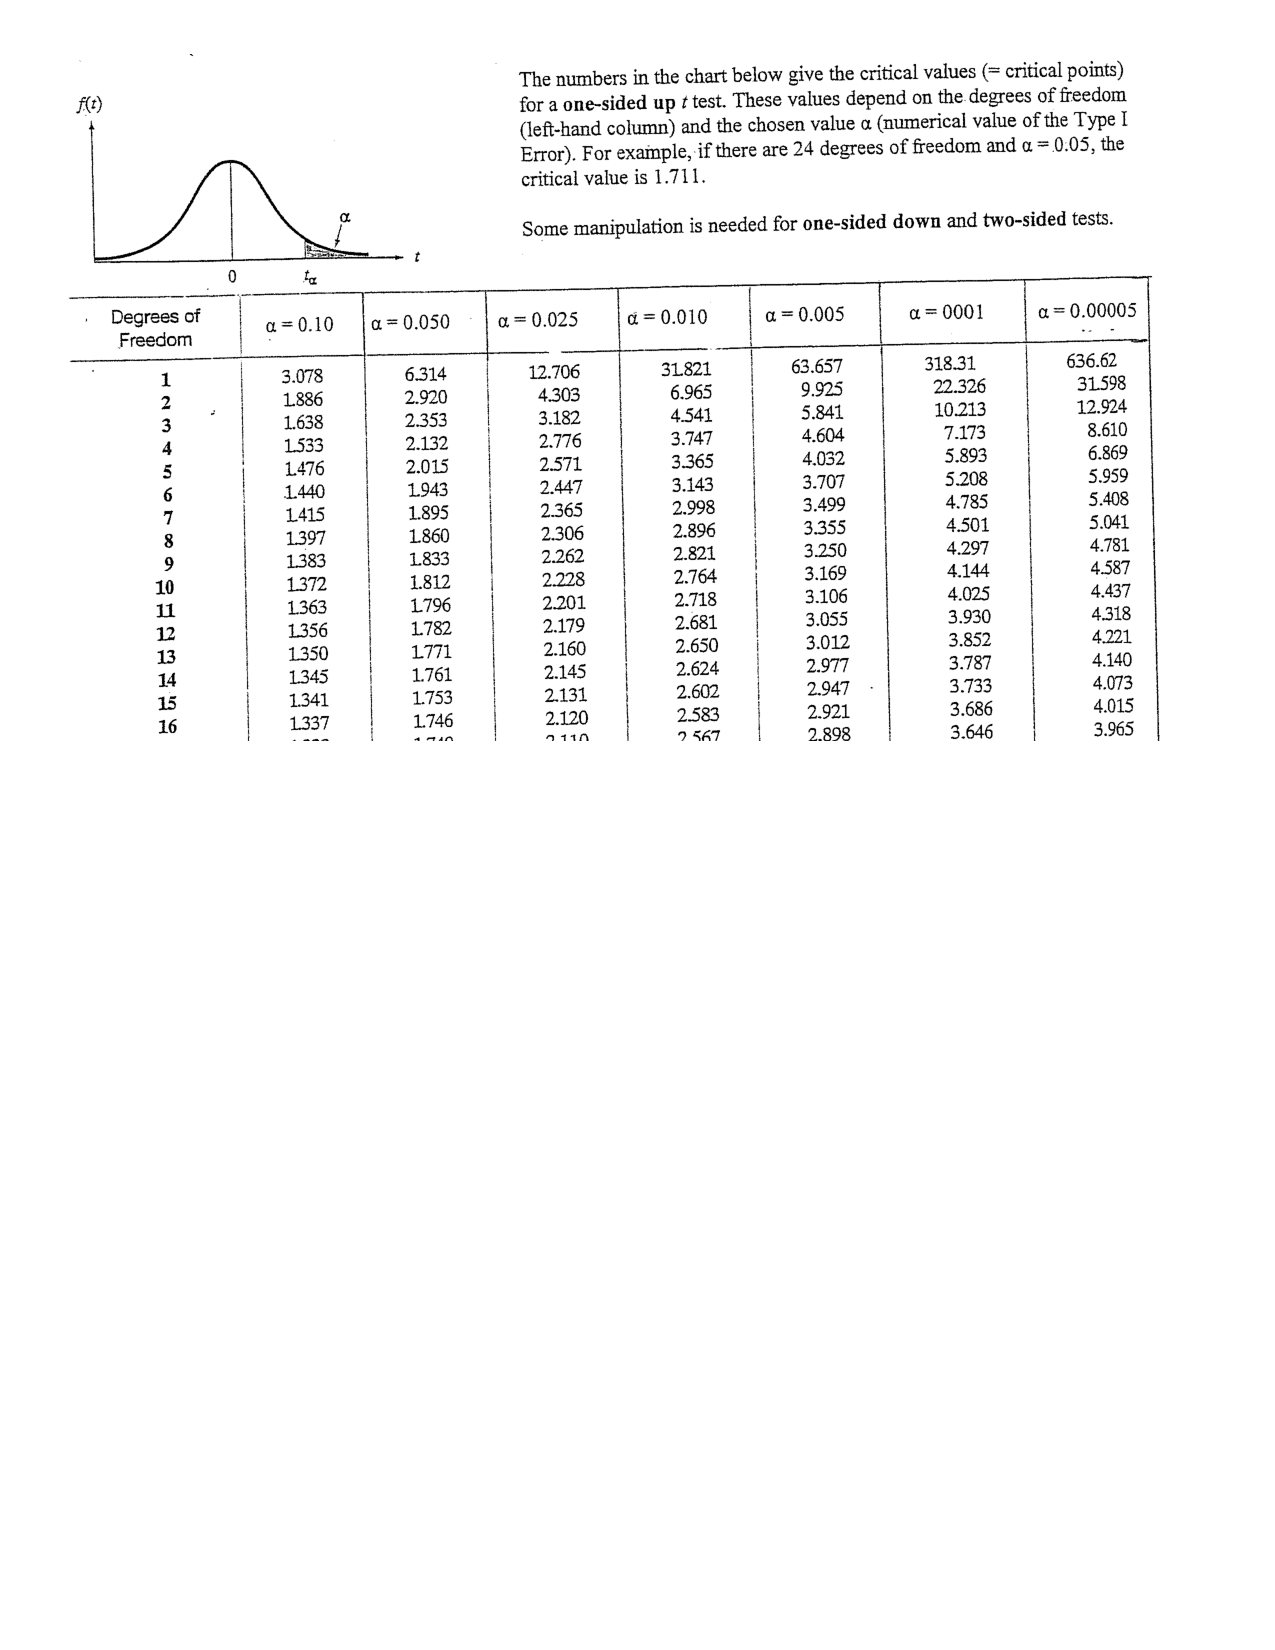
\includegraphics[width = 0.95\textwidth]{images/rec11_2}
\end{figure}
\uncover<2->{Here, the degrees of freedom is $n-1 = 14$. $P(t_{14} > 1.761) = 0.05 \text{ so } P(t_{14} < -1.761) = 0.05$ is the critical region}.
\end{frame}

\begin{frame}{Example}
\begin{itemize}
\setlength{\itemsep}{10pt}
\item A chocolate block is advertised as being 8 oz. Suppose we are concerned that the chocolate manufacturers are giving us less than 8 oz of chocolate in a block.  We collect 15 blocks of chocolate and calculate:
$$\bar{x} = 7.88, \quad s^2 = 0.06.$$
\item[Step 1] $H_0: \mu = 8$ vs. $H_1: \mu < 8$.   
\item[Step 2] Choose $\alpha = 0.05$. 
\item[Step 3] Test-statistic is 
$$t = \frac{\bar{x} - \mu_0}{s/\sqrt{n}} = \frac{7.88 - 8}{\sqrt{0.06/15}} = -1.90$$
\item[Step 4] Find the critical region $\Rightarrow t_{14} <-1.761$
\item<2->[Step 5] Since $t = -1.90$ is in the critical region, we reject $H_0$.
\end{itemize}
\end{frame}

\begin{frame}{Example}
\begin{figure}
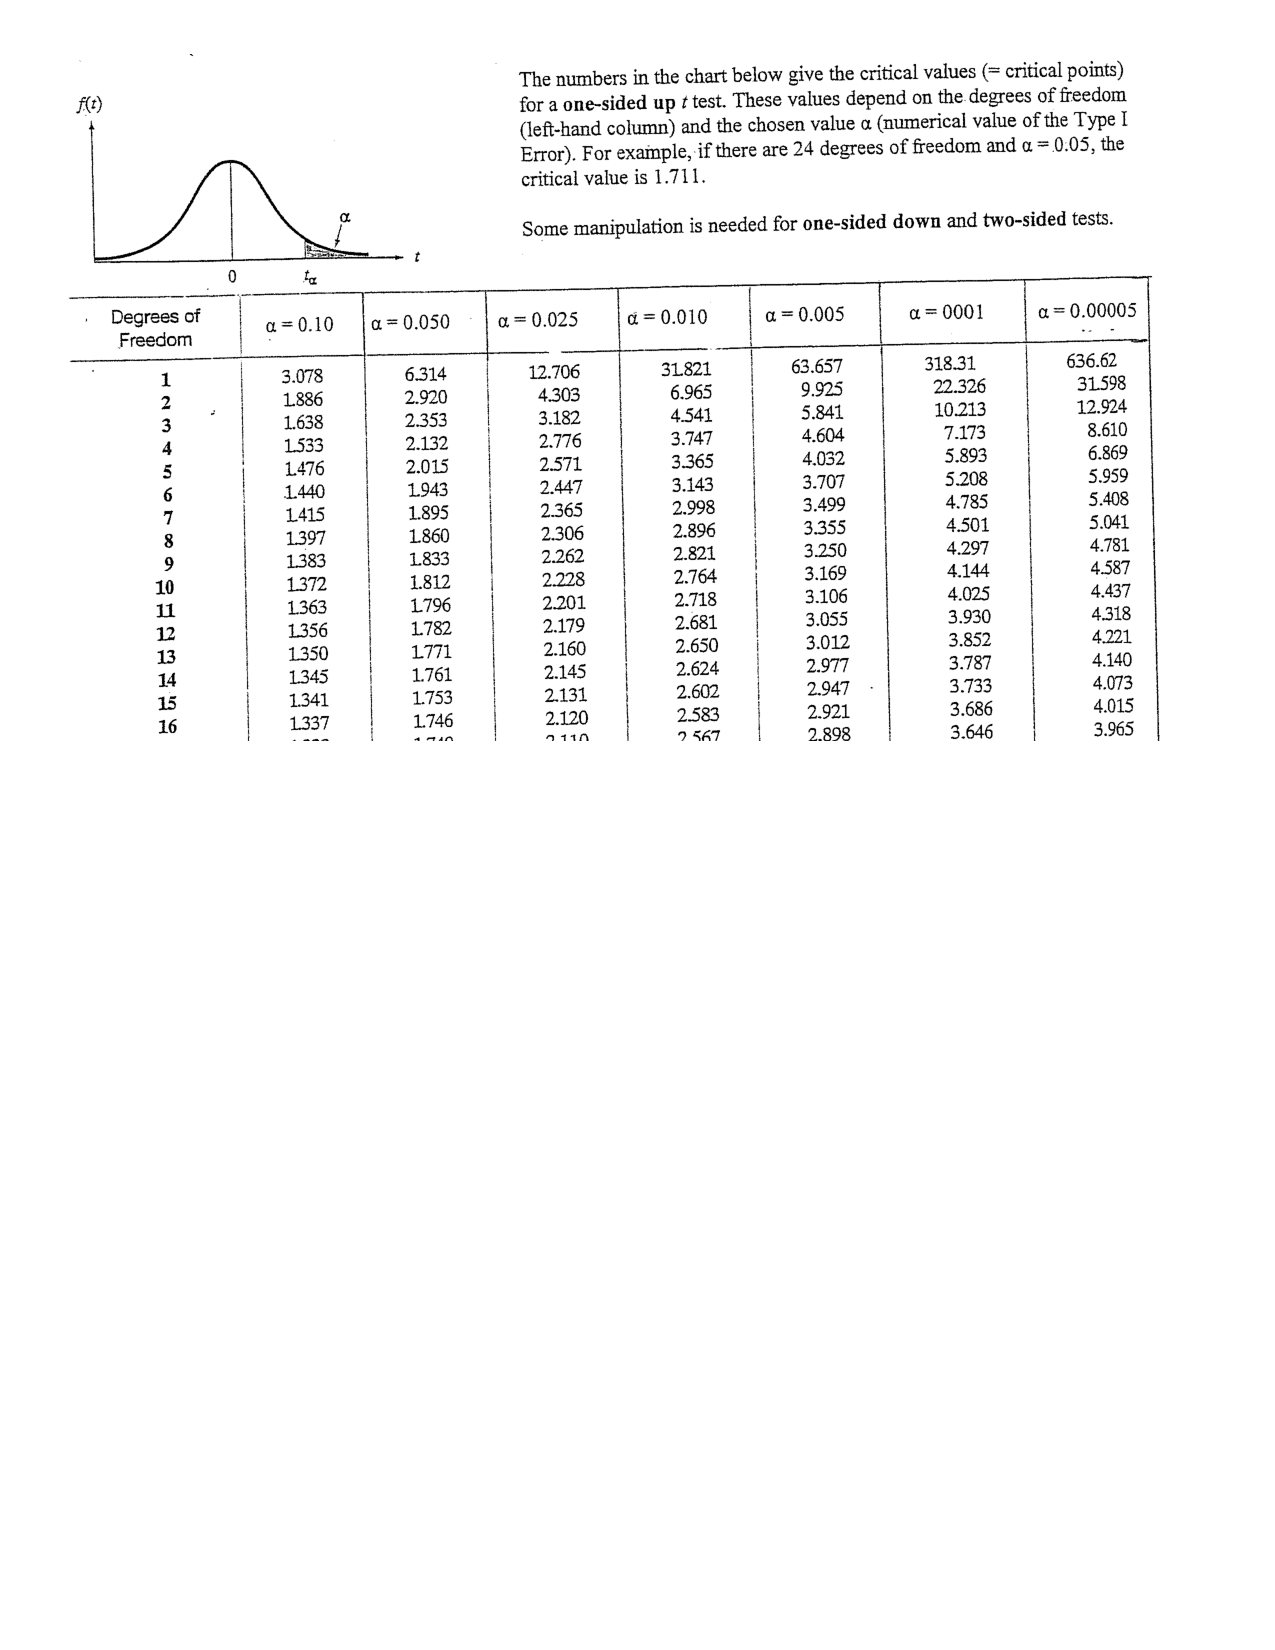
\includegraphics[width = 0.95\textwidth]{images/rec11_2}
\end{figure}
\small
\begin{itemize}
\setlength{\itemsep}{6pt}
\item For {\themecol one-sided} tests the critical region is: $t < -t_{n-1, \alpha}$ or $t > t_{n-1, \alpha}$ depending on the direction. 
\item For {\themecol two-sided} tests, the critical region is: $ t < -t_{n-1, \alpha/2} \text{ and }  t > t_{n-1, \alpha/2}.$
\end{itemize}
\end{frame}



\end{document}


